\documentclass[10pt]{article}
\usepackage{amssymb}
\usepackage{amsmath}
\usepackage{mathrsfs}
\usepackage{titlesec}
\usepackage{xcolor}
%\usepackage[shortlabels]{enumitem}
\usepackage{enumerate}
\usepackage{bm}
\usepackage{tikz}
\usepackage{listings}
\usetikzlibrary{arrows}
%\usepackage{subfigure}
\usepackage{graphicx,booktabs,multirow}
\usepackage[a4paper]{geometry}
\usepackage{upquote}
\usepackage{float}
\usepackage{pdfpages}

\usepackage[colorlinks,linkcolor=blue]{hyperref}
\usepackage{mdframed}

\usepackage{caption}
\graphicspath{{images/}}
\usepackage{subfig}

\iffalse
\usepackage{lastpage}
\usepackage{fancyhdr}
\fancyfoot[C]{Page \thepage\ of \pageref{LastPage}}
% Uncomment to remove the header rule
\renewcommand{\headrulewidth}{0pt} 
\pagestyle{fancy}
\fi

\geometry{verbose,tmargin=2cm,bmargin=2cm,lmargin=2cm,rmargin=2cm}
\geometry{verbose,tmargin=2cm,bmargin=2cm,lmargin=2cm,rmargin=2cm}
\lstset{language=Matlab}
\lstset{breaklines}

\input defs.tex

\newenvironment{solution}
    { \begin{mdframed}[backgroundcolor=gray!10] \textcolor{cyan}{\textbf{Solution}} \\}
    {  \end{mdframed}}

\newtheorem{proposition}{Proposition}
\newtheorem{remark}{Remark}

\titleformat*{\section}{\centering\LARGE\scshape}
\renewcommand{\thesection}{\Roman{section}}
\lstset{language=Matlab,tabsize=4,frame=shadowbox,basicstyle=\footnotesize,
keywordstyle=\color{blue!90}\bfseries,breaklines=true,commentstyle=\color[RGB]{50,50,50},stringstyle=\ttfamily,numbers=left,numberstyle=\tiny,
  numberstyle={\color[RGB]{192,92,92}\tiny},backgroundcolor=\color[RGB]{245,245,244},inputpath=code}

\begin{document}

%\title{CS150A--Database\\%
%	Final Exam Solutions}
%\date{}
%\maketitle


\section{Basics and SQL \textbf{[10 points]}}
\begin{enumerate}
	\item \textbf{[6 points]} \textbf{Basics} \\
	      For each sub-figure in Fig.~\ref{fig1}, select the letter corresponding to the best description. \\
	      A. Left Deep Tree \\
	      B. Key Compression \\
	      C. B+ Tree \\
	      D. Spark \\
	      E. Nested Loops Join \\
	      F. Sort Merge Join \\
	      G. Page Nested Loop Join \\
	      H. Slotted Page \\
	      I. Variable Length Tuple \\
	      J. Fixed Length Tuple \\
	      K. Buffer Frame \\
	      L. Sort-based Group-by \\
	      M. Recovery \\
	      N. Two Phase Lock \\
	      O. JSON \\
	      P. ISAM \\
	      Q. External Sort \\
	      R. MapReduce
	      \begin{figure}
		      \centering
		      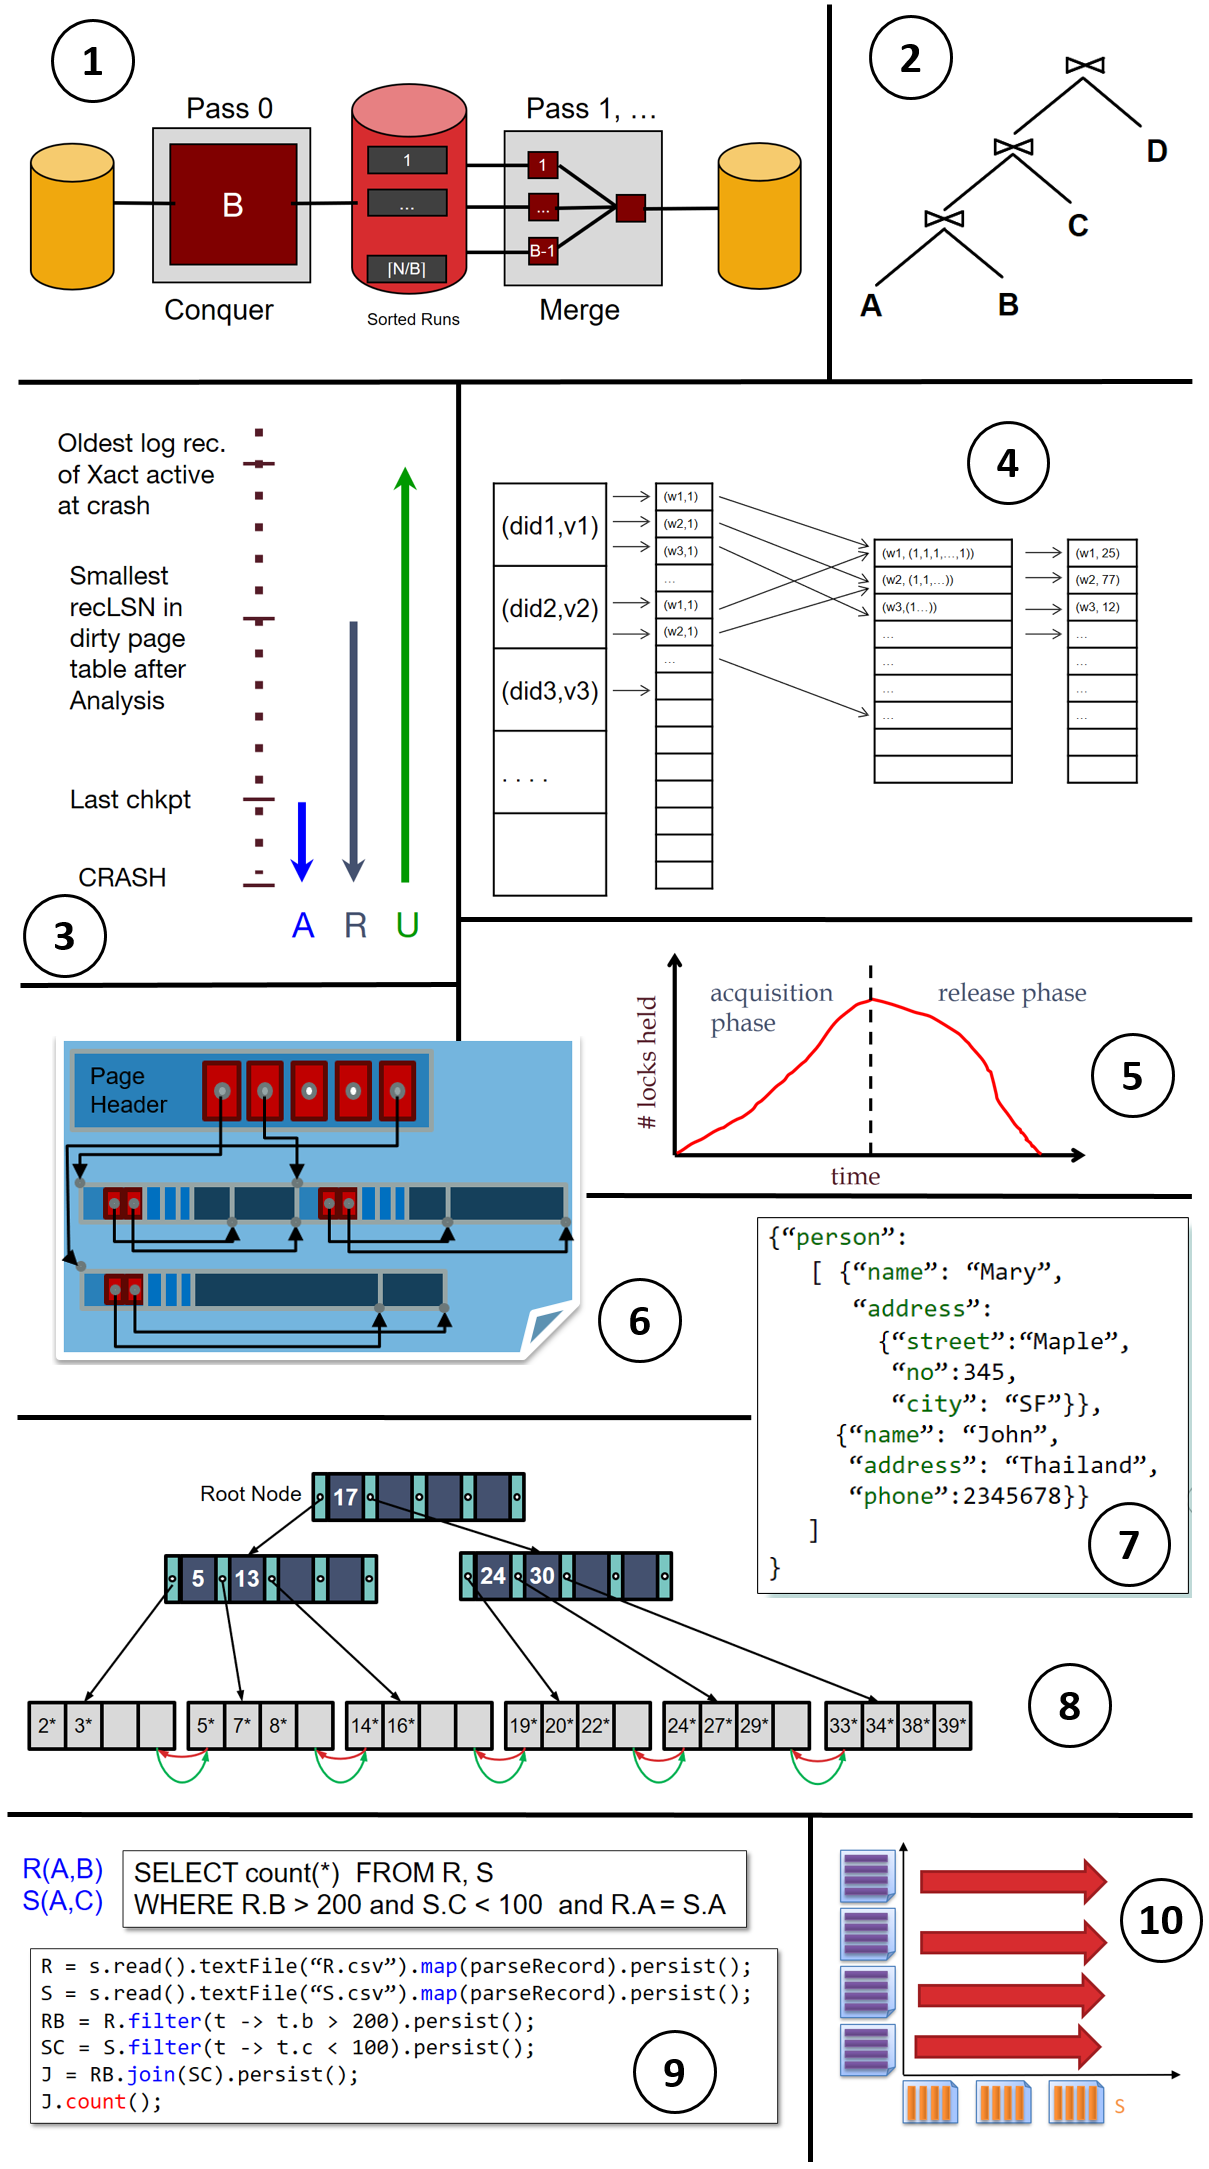
\includegraphics[width=.8\linewidth]{basics_new.png}
		      \caption{Basics of Database.}
		      \label{fig1}
	      \end{figure}
	      \newpage



	\item \textbf{[4 points]} \textbf{SQL} \\
	      Which of the following expressions computes the matrix vector product:
	      $$
		      (\mathbf{A} \mathbf{x})_{i}=\sum_{k=1}^{d} A_{i k} x_{k}
	      $$
	      Assume $\mathbf{A}$ and $\mathbf{x}$ have compatible dimensions and there is only one correct answer.\\
	      A.

	      \begin{lstlisting} 
SELECT A.row AS row, SUM(A.value * x.value) AS value 
FROM A JOIN x
ON A.col = x.row
GROUP BY A.row
\end{lstlisting}


	      B.
	      \begin{lstlisting}
SELECT A.row AS row, SUM(A.value * x.value) AS value 
FROM A JOIN x
ON A.row = x.row
GROUP BY A.col
\end{lstlisting}
	      C.
	      \begin{lstlisting} 
SELECT x.row AS row, SUM(A.value * x.value) AS value 
FROM A JOIN x
ON A.col = x.row
GROUP BY A.col
\end{lstlisting}
	      D.
	      \begin{lstlisting}
SELECT A.row AS row, A.value * x.value AS value 
FROM A JOIN x
ON A.row = x.row  
\end{lstlisting}

\end{enumerate}
\textbf{Your answer:}




\newpage
\section{B+ Trees and Buffer Management \textbf{[10 points]}}

\begin{enumerate}


	\item \textbf{[4 points]} \textbf{Index and B+ Trees} \\
	      Consider the following B+ tree of order 2. \\
	      (Note: correct answer without appropriate explanation would earn zero score.)
	      \begin{center}
		      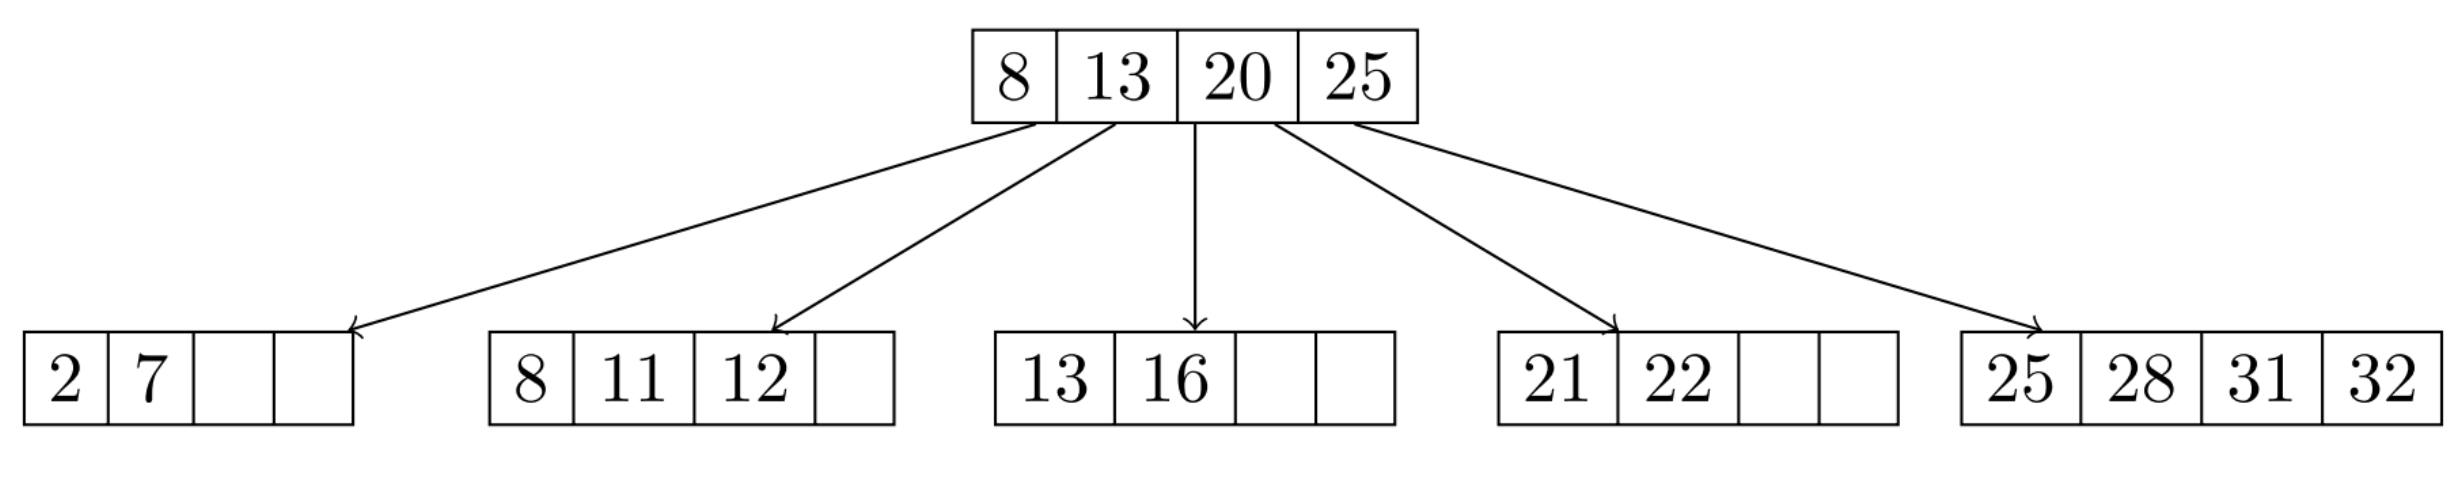
\includegraphics[scale=0.25]{Btree.png}
	      \end{center}
	      \begin{itemize}
		      \item[(a)] \textbf{[2 points]} How many nodes split when you insert 27? \\

		      \item[(b)] \textbf{[2 points]} After inserting 27 into the tree, you also insert 26, how many nodes split as a result of inserting 26? \\

	      \end{itemize}


	\item \textbf{[6 points]} \textbf{Buffer Management} \\
	      Supposed we have a buffer pool size of 4 pages, and the following access pattern: \\
	      A P P L E S A N D B A N A N A S A N D O R A N G E S \\
	      Assume that pages are unpinned immediately (ignore pinning), and we are starting from a cold (empty) cache.
	      \begin{itemize}
		      \item[(a)] \textbf{[2 points]} What is the number of cache hits if we
		            use an LRU replacement policy? \\

		      \item[(b)] \textbf{[2 points]} What is the number of cache hits if we
		            use an MRU replacement policy? \\

		      \item[(c)] \textbf{[2 points]} What is the number of cache hits if we
		            use a CLOCK replacement policy?  \\

	      \end{itemize}
\end{enumerate}
\textbf{Your answer:}


\newpage
\section{Sorting and Join Algorithms \textbf{[10 points]}}
\begin{enumerate}

	\item \textbf{[4 points]}  \textbf{External Sorting} \\
	      Assume that each page is 4 KB large, and that you have a 24KB buffer pool (with 6 frames).
	      \begin{itemize}
		      \item[(a)] \textbf{[2 points]} How many passes would it take to externally sort an 512KB file?
		            Include the initial sorting pass and subsequent merging passes in your answer. You need to simplify your answer. \\

		      \item[(b)] \textbf{[2 points]} What would be the total cost in I/Os for this external sort? \\

	      \end{itemize}


	\item \textbf{[6 points]} \textbf{Join Algorithms} \\
	      Consider a new case, i.e. B$>$4 pages worth of buffer space, and relations M and N of size $>$ B.
	      Please fill the blanks below with ``always'', ``sometimes'' or ``never''.
	      \begin{itemize}
		      \item[(a)] \textbf{[2 points]} Block nested loop join is \underline{\ \ \ \ \ \ \ \ \ \ } better than page-oriented nested loop join. \\

		      \item[(b)] \textbf{[2 points]} Sort-merge join is \underline{\ \ \ \ \ \ \ \ \ \ } better than hash-join. \\

		      \item[(c)] \textbf{[2 points]} Hybrid Hash-Join is \underline{\ \ \ \ \ \ \ \ \ \ } better than block-nested loops join. \\

	      \end{itemize}
\end{enumerate}
\textbf{Your answer:}


\newpage
\section{Transactions and Concurrency \textbf{[10 points]}}

\begin{enumerate}

	\item \textbf{[6 points]} \textbf{Transactions} \\
	      Consider the following schedule. (For each of the questions below, you may mark zero ($\phi$), one
	      or more than one of the choices.)
	      \begin{center}
		      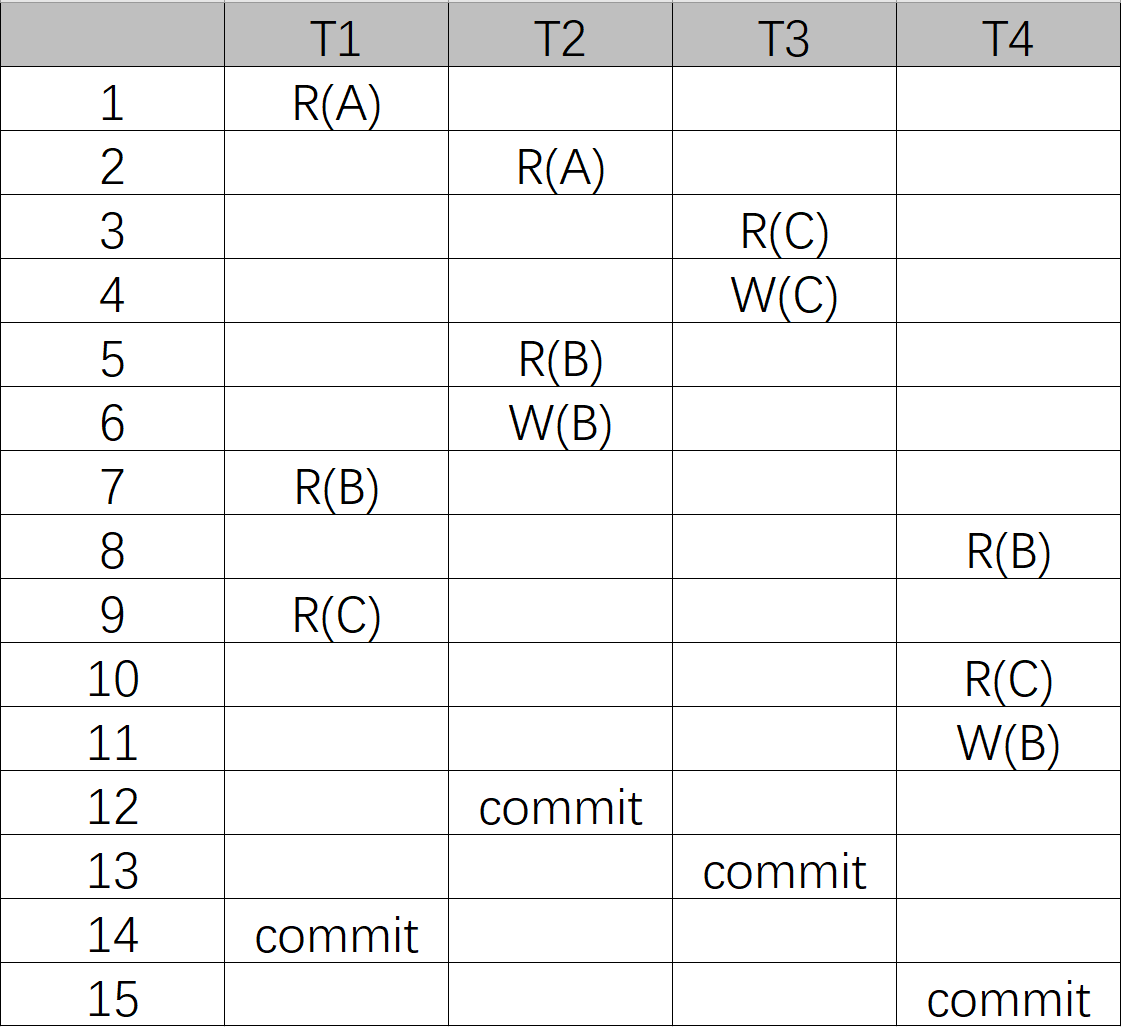
\includegraphics[scale=0.35]{transaction}
	      \end{center}
	      \begin{itemize}
		      \item[(a)] \textbf{[2 points]} Please draw the conflict dependency graph of the above schedule?\\

		      \item[(b)] \textbf{[2 points]} Which of the following schedules below are conflict equivalent to the schedule above?\\
		            A. T3, T1, T2, T4\\
		            B. T2, T3, T1, T4\\
		            C. T4, T3, T1, T2\\
		            D. T1, T2, T3, T4 \\

		      \item[(c)] \textbf{[2 points]} Select one or more than one true statement(s): \\
		            A. In Strict 2PL, we can give up locks after aborting but before rollback
		            is complete. \\
		            B. Schedules that are conflict serializable can not produce a cyclic
		            dependency graph. \\
		            C. 2PL does not promise conflict serializability. \\
		            D. Strict Two Phase Locking ensures that we do not have deadlocks. \\

	      \end{itemize}

	\item \textbf{[4 points]} \textbf{Lock Manager} \\
	      Given the database system shown below:
	      \begin{figure}[ht]
		      \centering
		      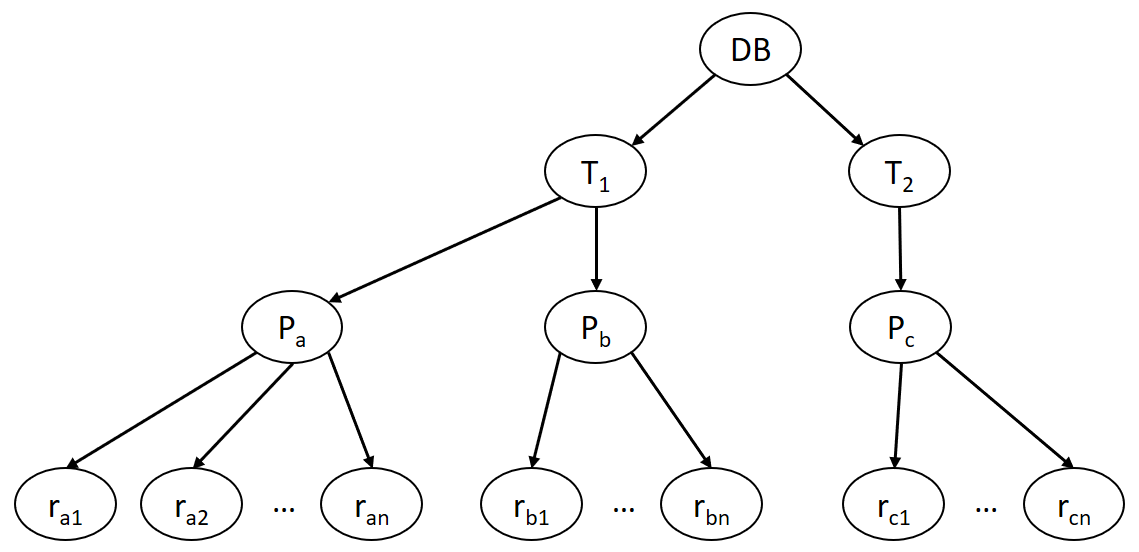
\includegraphics[width=0.7\linewidth]{lock_mode}
	      \end{figure}
	      \begin{itemize}
		      \item[(a)] \textbf{[2 points]} Which lock modes (including S, X, IS, IX, or SIX) on which resources are necessary to read $P_a$? \\
		      \item[(b)] \textbf{[2 points]} Which lock modes (including S, X, IS, IX, or SIX) held by other transactions on $P_a$ would prevent us from modifying $r_{a1}$? \\
	      \end{itemize}

\end{enumerate}
\textbf{Your answer:}


\newpage
\section{Logging and Recovery \textbf{[10 points]}}

\begin{enumerate}
	\item \textbf{[4 points]} \textbf{Basics} \\
	      Select the correct choices in the following questions:
	      \begin{itemize}
		      \item[(a)] Write Ahead Logging describes a protocol where updated pages must be written to disk before a crash. \\
		            A. True \\
		            B. False \\
		      \item[(b)] During a transaction abort, we undo all data updates made by the transaction. \\
		            A. True \\
		            B. False \\
		      \item[(c)] In ARIES, UPDATE log records contain no information of the previous state of the page. \\
		            A. True \\
		            B. False \\
		      \item[(d)] The recovery manager is responsible for Atomicity and Consistency, as defined by the ACID acronym. \\
		            A. True \\
		            B. False \\
		      \item[(e)] If PageLSN is greater than the max LSN flushed so far (flushedLSN), we can safely write this page to disk. \\
		            A. True \\
		            B. False \\
		      \item[(f)] In ARIES recovery, after the analysis phase, the recLSN of each page in the dirty page table must be larger than the pageLSN of the corresponding page. \\
		            A. True \\
		            B. False \\
		      \item[(g)] When aborting a transaction, it is necessary to modify pages on disk. \\
		            A. True \\
		            B. False \\
		      \item[(h)] Write-Ahead Logging (WAL) guarantees that a transactions log records are flushed to disk before the transaction commit. \\
		            A. True \\
		            B. False \\
	      \end{itemize}
		  
\newpage
	\item \textbf{[6 points]} \textbf{Recovery} \\
	      Your database server has just crashed due to a power outage.
	      You boot it back up, find the following log and checkpoint information on disk,
	      and begin the recovery process. Assume we use a STEAL/NO FORCE recovery policy.
	      \begin{figure}[h]
		      \centering
		      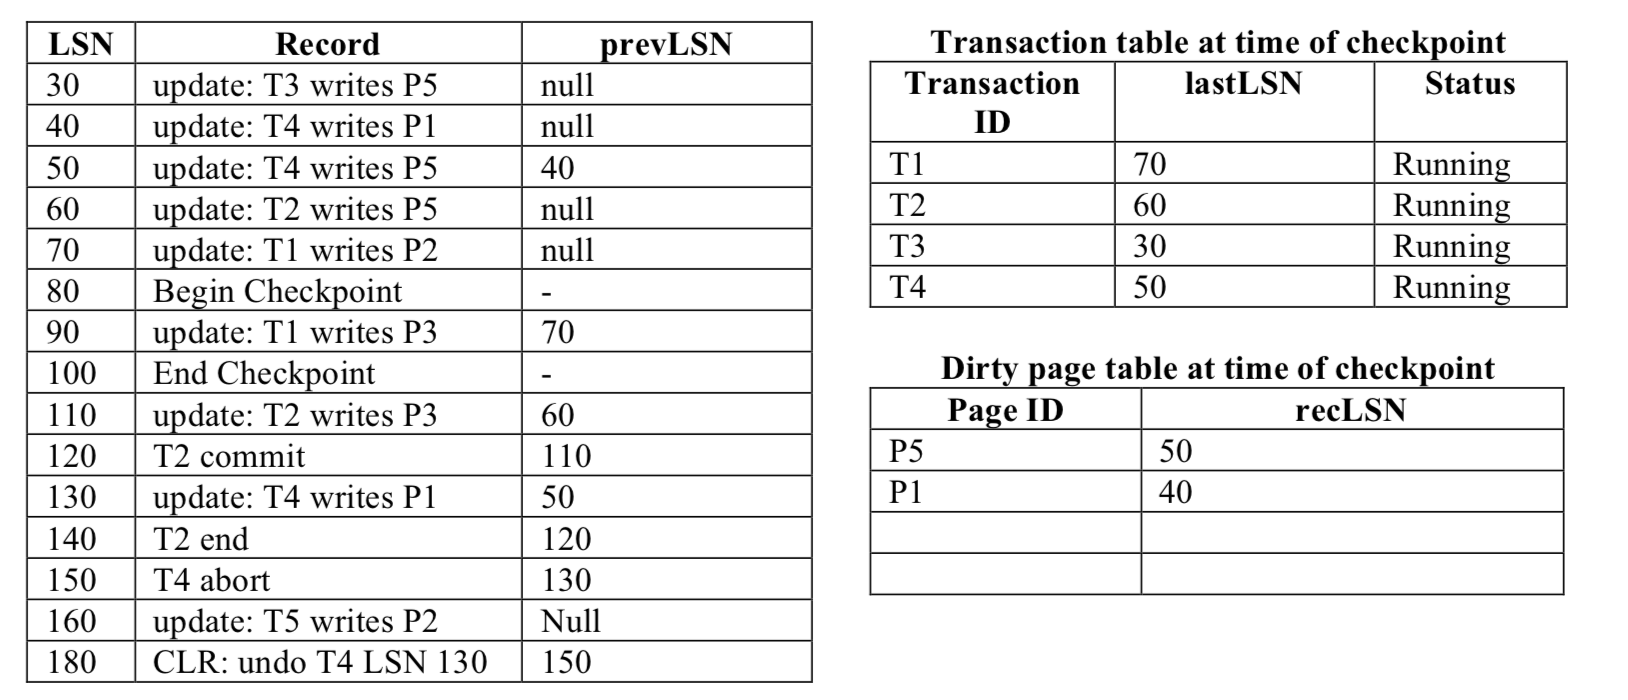
\includegraphics[width=.8\linewidth]{recovery}
		      %	\caption{Logging and recovery}
		      \label{fig:recovery}
	      \end{figure}
	      \begin{itemize}
		      \item[(a)] \textbf{[3 points]}
		            At the end of the Analysis phase, what transactions will be in the transaction table,
		            and with what lastLSN and Status values?
		            We also accept the answer by moving the status of transactions in the above table from ``Running'' to ``Aborting''. \\
		      \item[(b)] \textbf{[3 points]}
		            At the end of the Analysis phase, what pages will be in the dirty page table, and with what recLSN values? \\
	      \end{itemize}

\end{enumerate}
\textbf{Your answer:}



\newpage
\section{Database Design \textbf{[10 points]}}

\begin{enumerate}

	\item \textbf{[4 points]} \textbf{ER Modeling} \\
	      In this question, we will choose to model elements of a baseball league using ER-Diagrams. We have 4 entities:
	      \textbf{Supporter}, \textbf{Team}, \textbf{Player} and \textbf{Agent}. Refer to the Figure below for the following questions.
	      \begin{figure}[ht]
		      \centering
		      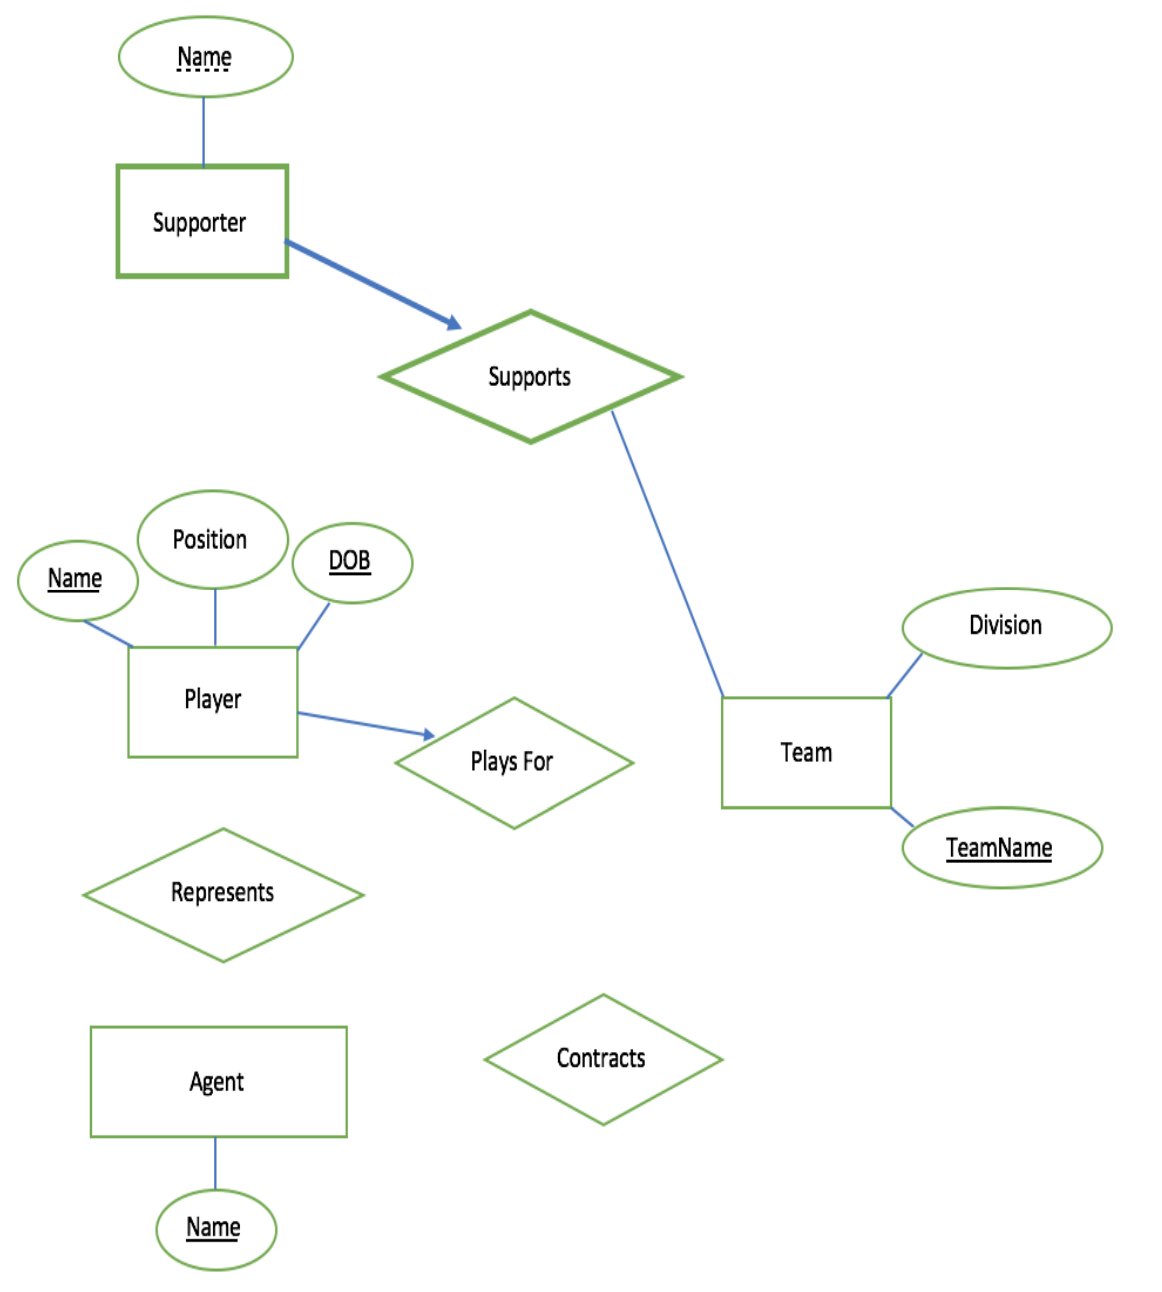
\includegraphics[width=0.7\linewidth]{pro2}
		      \caption{ER model}
		      \label{fig_pro2}
	      \end{figure}

	      \begin{enumerate}
		      \item \textbf{[3 points]} There are some elements of the ER-diagram are missing in Fig.~\ref{fig_pro2},
		            fill them in so that the ER-diagram satisfies the following constraints.
		            \begin{itemize}
			            \item Each team must have at least one player on its roster.
			            \item Each player must have exactly one agent to represent him/her.
			            \item Each agent can sign as many contracts as he or she wants to, or none at all.
			            \item Each player can have at most one contract.
			            \item A team has at least one contract.
			            \item Relation \textbf{Represents} involves entities \textbf{Player} and \textbf{Agent}; relation \textbf{Contracts} involves
			                  entities \textbf{Player}, \textbf{Agent} and \textbf{Team}; relation \textbf{Plays For} involves entities \textbf{Team} and \textbf{Player}
		            \end{itemize}
		            (Hint: you should add 6 edges in total.) \\

		      \item \textbf{[1 point]} As \textbf{Supporter} is a weak entity that must have unique and total participation in the \textbf{Supports} relation,
		            its primary key is determined by which attribute(s) in the ER-diagram? \\
		            A. Name \\
		            B. TeamName \\
		            C. Name, TeamName \\
		            D. None of them \\

	      \end{enumerate}


	\item \textbf{[3 points]} \textbf{Functional Dependencies} \\
	      We have a relation R(A, B, C, D, E). We are told that the set of functional dependencies is
	      F = {E → BC, A → B, C → D, AD → C}.
	      \begin{itemize}
		      \item[(a)] \textbf{[1 point]} What are A+, C+ and E+? \\
		      \item[(b)] \textbf{[1 point]} Is the attribute set ACE the superkey for relation R? \\
		      \item[(c)] \textbf{[1 point]} Is relation R already in Boyce-Codd Normal Form (BCNF)? \\
	      \end{itemize}


	\item \textbf{[3 points]} \textbf{Normalization and Decomposition} \\
	      Decompose ABCDEFGH into Boyce-Codd Normal Form (BCNF) in the order of the following FDs:
	      G → H; EF → B; EA → C; FH → D. \\

\end{enumerate}
\textbf{Your answer:}


\newpage
\section{Parallel Query Processing \textbf{[10 points]}}

\begin{enumerate}

	\item \textbf{[4 points]} \textbf{Partition} \\
	      Assume that we have 5 machines and a 1000 page \textbf{students(sid, name, gpa)} table. Initially,
	      all of the pages start on one machine. Assume each page is 1KB.
	      \begin{itemize}
		      \item[(a)] \textbf{[2 points]} How much network cost does it take to round-robin partition the table? \\
		      \item[(b)] \textbf{[2 points]} How many IOs will it take to execute the following query:
		            \begin{lstlisting} 
  SELECT *
  FROM students
  WHERE name = 'John'
\end{lstlisting}
	      \end{itemize}


	\item \textbf{[6 points]} \textbf{Parallel Algorithm} \\
	      Assume that we have a 100 page table R that we will join with a 400 page table S.
	      All the pages start on machine 1, and there are 4 machines in total with 30 buffer pages each.
	      \begin{itemize}
		      \item[(a)] \textbf{[2 points]} How many passes are needed to do a parallel unoptimized Sort-Merge Join (SMJ) on the data? For
		            this question a pass is defined as a full pass over either table (so if we have to do 1 pass over R and 1 pass
		            over S it is 2 total passes). \\
		      \item[(b)] \textbf{[2 points]} How many passes are needed to a parallel Grace Hash Join on the data? \\
		      \item[(c)] \textbf{[2 points]} We want to calculate the max in parallel using hierarchical aggregation. What value should
		            each machine calculate and what should the coordinator do with those values? \\
	      \end{itemize}

\end{enumerate}
\textbf{Your answer:}




\newpage
\section{Distributed Transactions and NoSQL \textbf{[10 points]}}

\begin{enumerate}
	\item \textbf{[3 points]} \textbf{2-Phase Commit} \\
	      Select the correct choices in the following questions:
	      \begin{itemize}
		      \item[(a)] If we are recovering and see a PREPARE record, it means we must have sent out a YES vote. \\
		            A. True \\
		            B. False \\
		      \item[(b)] If the coordinator is recovering and sees a COMMIT record, we can locally commit and end the process there. \\
		            A. True \\
		            B. False \\
		      \item[(c)] Suppose a participant receives a prepare message for a transaction and replies VOTE-YES.
		            Suppose that they were running a wound-wait deadlock avoidance policy, and a transaction
		            comes in with higher priority. The new transaction will abort the prepared transaction. \\
		            A. True \\
		            B. False \\
	      \end{itemize}

	\item \textbf{[2 points]} \textbf{OLTP and OLAP} \\
	      Are the following workloads better characterized as Online Transaction Processing (OLTP)
	      or Online Analytical Processing (OLAP)? Select the correct choices in the following questions:
	      \begin{itemize}
		      \item[(a)] Placing orders and buying items in an online marketplace. \\
		            A. OLTP \\
		            B. OLAP \\
		      \item[(b)] Analyzing trends in purchasing habits in an online marketplace. \\
		            A. OLTP \\
		            B. OLAP \\
	      \end{itemize}


	\item \textbf{[5 points]} \textbf{NoSQL} \\
	      Select the correct choices in the following questions:
	      \begin{itemize}
		      \item[(a)] As methods for scaling dataset, partitioning is effective for write-heavy workloads, and replication is effective for read-heavy workloads.  \\
		            A. True \\
		            B. False \\
		      \item[(b)] Partitioning and replication are often used together in real systems to leverage the performance
		            benefits and to make the system more fault-tolerant. \\
		            A. True \\
		            B. False \\
		      \item[(c)] The consistency in the distributed systems is the same concept with the consistency found in ACID (Transactions). \\
		            A. True \\
		            B. False \\
		      \item[(d)] JSON and XML are referred as semi-structured data formats, and can express complex data structures, which may be arranged into nested structures. \\
		            A. True \\
		            B. False \\
		      \item[(e)] JSON is self-describing, and it is designed for efficient storage and retrieval from disk. \\
		            A. True \\
		            B. False \\
	      \end{itemize}

\end{enumerate}
\textbf{Your answer:}
%\newpage\phantom{blabla}

\newpage
\section{MapReduce and Spark \textbf{[10 points]}}

\begin{enumerate}

	\item \textbf{[3 points]} \textbf{Basics} \\
	      Select all the true statement(s): \\
	      A. In MapReduce, the Map phase applies a function in parallel to every element of a set of data, and the Reduce phase combines the
	      results of the Map phase into the desired data output. \\
	      B. In Distributed File System (DFS), a file system in which large files are partitioned into smaller files,
	      and then distributed and replicated several times on different nodes for fault tolerance. \\
	      C. Both the Map and Reduce phases can be split among different
	      workers on different machines, with workers performing independent tasks in parallel. \\
	      D. Since the Reduce phase must wait until the entire Map phase completes, we must restart the entire Map phase if one map task
	      fails. \\
	      E. Resilient Distributed Datasets (RDDs) are not written to disk in intermediate steps but are rather stored in main memory. \\
	      F. Similar with MapReduce, Spark needs to write intermediate results to disk. \\

	\item \textbf{[7 points]} \textbf{MapReduce} \\
	      \begin{itemize}
		      \item[(a)]  \textbf{[2 points]}  Fig.~\ref{mr1} shows a relation $R(A)$ with the MapReduce implementation of the Selection operator $\sigma_{A=123}(R)$.
		            \begin{figure}[H]
			            \centering
			            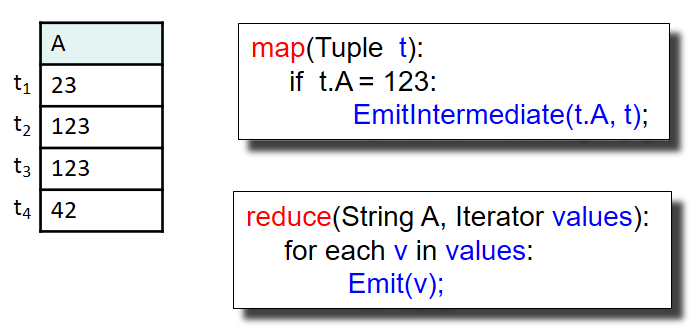
\includegraphics[width=0.5\linewidth]{mr_selection}
			            \caption{Selection}
			            \label{mr1}
		            \end{figure}
		            \begin{itemize}
			            \item[(1)] What is the output of the Map function?
			            \item[(2)] What is the output of the Reduce function? \\
		            \end{itemize}
		      \item[(b)] \textbf{[2 points]}  Fig.~\ref{mr2} shows a relation $R(A,B)$ with the MapReduce implementation of the Group-By operator $\gamma_{A=123,\text{SUM} (B)}(R)$.
		            \begin{figure}[H]
			            \centering
			            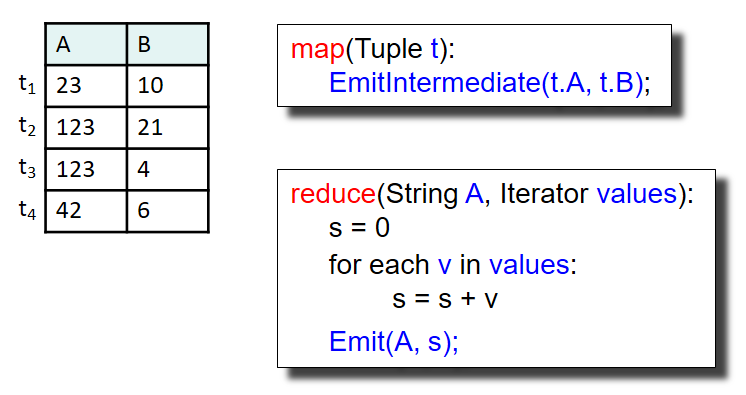
\includegraphics[width=0.5\linewidth]{mr_group}
			            \caption{Group-By}
			            \label{mr2}
		            \end{figure}
		            \begin{itemize}
			            \item[(1)] What is the output of the Map function?
			            \item[(2)] What is the output of the Reduce function? \\
		            \end{itemize}
		      \item[(c)] \textbf{[3 points]}  Fig.~\ref{mr3} shows two relations $R(A,B)$ and $S(C,D)$ with the MapReduce implementation of the Hash-Join operator $R(A,B) \bowtie_{B=C} S(C,D)$.
		            \begin{figure}[H]
			            \centering
			            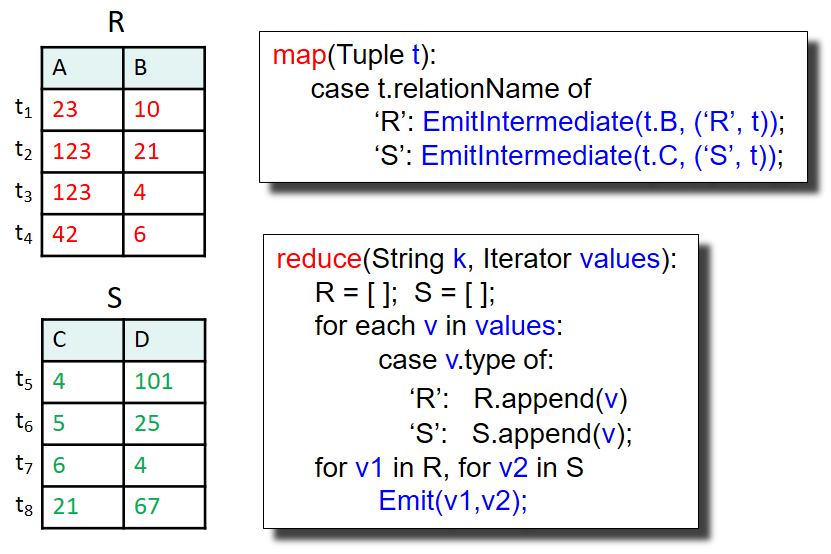
\includegraphics[width=0.55\linewidth]{mr_join}
			            \caption{Hash-Join}
			            \label{mr3}
		            \end{figure}
		            \begin{itemize}
			            \item[(1)] What is the output of the Map function?
			            \item[(2)] What is the output of the Reduce function? \\
		            \end{itemize}
	      \end{itemize}

\end{enumerate}
\textbf{Your answer:}


\newpage
\section{Data Mining and Machine Learning \textbf{[10 points]}}

\begin{enumerate}

	\item \textbf{[2 points]} \textbf{Basics} \\
	      Select all the true statement(s): \\
	      A. The order of the basic KDD (Knowledge Discovery in Database) process is Data Selection, Data Cleaning, Data Mining \& ML, Evaluation. \\
	      B. The ultimate goal in machine learning is to find a model that best fits the training data. \\
	      C. The $k$-means algorithm is guaranteed to converge to the global optimum. \\
	      D. A common form of feature engineering on continuous data is one-hot-encoding. \\

	\item \textbf{[4 points]} \textbf{K-Means}
	      \begin{itemize}

		      \item[(a)] \textbf{[2 points]}
		            Which of the following can act as possible termination conditions in $k$-means?
		            (you may select one or more than one of the choices.)\\
		            A. For a fixed number of iterations.\\
		            B. Assignment of observations to clusters does not change between iterations. Except for cases with a bad local minimum.\\
		            C. Centroids do not change between successive iterations.\\
		            D. Terminate when the objective value falls below a threshold. \\


		      \item[(b)] \textbf{[2 points]}
		            In which of the following cases will $k$-means clustering fail to give good results?
		            (you may mark zero ($\phi$), one or more than one of the choices.)\\
		            A. Data points with outliers.\\
		            B. Data points with different densities.\\
		            C. Data points with round shapes.\\
		            D. Data points with non-convex shapes. \\

	      \end{itemize}



	\item \textbf{[4 points]} \textbf{Linear Regression} \\
	      Given $n$ independent and identically distributed (i.i.d.) training samples
	      $\{(x_1, y_1), (x_2, y_2), ... , (x_n, y_n)\}$, with the $i$-th sample $x_i, y_i \in \mathbb{R}$, $i=1,2,...,n$.
	      Consider the linear model:
	      \begin{equation}
		      y = x\theta + \epsilon \quad \epsilon\sim\mathcal{N}(0,\,\sigma^{2}),
	      \end{equation}
	      where $\mathcal{N}(0,\,\sigma^{2})$ denotes the Guassian distribution with mean 0 and variance $\sigma^2$.
	      Assume that the training data has been centralized, such that the intercept can be ignored in the above linear model.
	      Obviously, the probability density function of $y$ conditioned on $x$ and $\theta$ follows the Gaussian distribution $\mathcal{N}(x\theta,\sigma)$,
	      which is defined by
	      \begin{equation}
		      p(y|x,\theta) = \frac{1}{\sqrt{2\pi\sigma^2}}\exp(-\frac{1}{2\sigma^2}(y-x\theta)^2).
	      \end{equation}
	      The model parameter $\theta$ can be estimated based on Maximum Likelihood Estimation (MLE), which aims to maximize the likelihood function:
	      \begin{align}
		      L(\theta) & = \prod_{i=1}^n P(x_i,y_i|\theta) \nonumber                                                    \\
		                & = \prod_{i=1}^n P(y_i|x_i,\theta)P(x_i) \nonumber                                              \\
		                & = \prod_{i=1}^n \frac{1}{\sqrt{2\pi}\sigma}\exp(-\frac{(y_i - x_i\theta)^2}{2\sigma^2})P(x_i).
	      \end{align}
	      (Hint: $P(x_i)$ ($i=1,2,...,n$) can be treated as a constant in the above formulation.)
	      \begin{itemize}
		      \item[(a)] \textbf{[2 points]} Show the log-likelihood function $\log L(\theta)$. (The base of the log function is $e$.) \\
		      \item[(b)] \textbf{[2 points]} Apply MLE to calculate the closed-form solution of $\theta$. \\
	      \end{itemize}

\end{enumerate}
\newpage
\textbf{Your answer:}
%\newpage\phantom{blabla}

\end{document}